\documentclass[compress, darktitle, framenumber, mathserif]{beamer}
\usepackage{pgfplots}
\usepackage{tikz}
\usepackage{xparse}
\usepackage{graphicx}
\usepackage{epsfig}
\usepackage{float}
\restylefloat{figure}
\restylefloat{table}
\usepackage[font=small,format=plain,labelfont=bf,up,textfont=it,up]{caption}

\usepackage[dutch]{babel}
\usepackage{enumerate}

%\usepackage[usenames,dvipsnames]{color}

\usepackage{amsmath,amsfonts,amsthm,amssymb}
\usepackage{mathrsfs}
\usepackage{mathtools}
\usepackage{accents}
\usetikzlibrary{matrix,arrows}

\mathtoolsset{showonlyrefs}

\usetheme{UniversiteitAntwerpen}

\title{Wisku$\mathbb{N}$de in-$\mathbb{Z}$icht}
\subtitle{Wiskunde in muziek}
\author{Pieter Belmans (\texttt{pieter.belmans@uantwerpen.be}) \\ Matthias Roels (\texttt{matthias.roels@uantwerpen.be})}
\date{9 januari 2014}

%%%%%%%%%%%%%%%%%%%%%%%%%%%%%%%%%%%
%%%%%%%%%%Commando's Matthias%%%%%%%%%

\newcommand{\comm}[1]{\lbrack #1 \rbrack} %notatie van Lie haak
\newcommand{\set}[1]{\left\{ #1 \right\} } %notatie voor haakjes voor een verzameling
\newcommand{\brac}[1]{\left( #1 \right)} %notatie voor haakjes

\newcommand{\R}{\mathbb{R}} % the field of the reals
\newcommand{\N}{\mathbb{N}} % the field of the natural numbers
\newcommand{\C}{\mathbb{C}} % the field of complex number
\newcommand{\Z}{\mathbb{Z}} % the field of integers


\begin{document}
\begin{frame}
  \titlepage
\end{frame}

\begin{frame}
\frametitle{Wat is geluid}
\begin{itemize}
\item Geluid is een periodisch signaal (een ``golf '') 
\item Wiskundig: een functie die afhangt van de tijd zodat $$f(t+P)=f(t),$$ met $P$ de periode.
\item Hoe beschrijft men deze functies? 
\end{itemize}
\end{frame}

\begin{frame}
\frametitle{Wat zijn de meest eenvoudige signalen?}
\begin{itemize}
\item Dit zijn de zgn. goniometrische functies $$f(t)=A\cos (\omega t) \quad \text{en} \quad g(t)=B\sin (\omega t),$$ met $A$ en $B$ de amplitude en $\omega$ de frequentie. 
\item Amplitude: $\frac{1}{2}$(het verschil tussen piek en dal)
\item Frequentie: $($afstand tussen twee toppen van de golf$)^{-1}$
\item Kunnen we deze gebruiken om complexere signalen te beschrijven?  
\end{itemize}
\end{frame}

\begin{frame}[fragile]
\frametitle{Een analogie met vectoren}
\begin{itemize}
\item Een vector kan geschreven worden als $\vec{v}=a\vec{e}_x+b\vec{e}_y.$
\end{itemize}
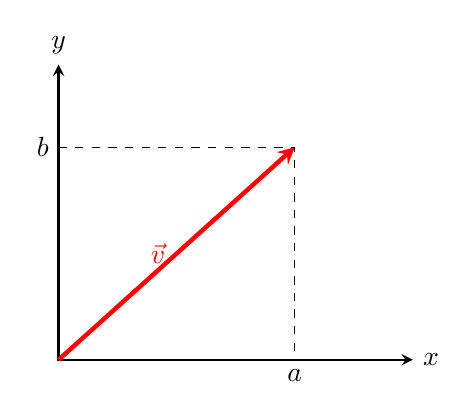
\begin{tikzpicture}[scale=1.5]
    % Draw axes
    \draw [>=stealth,<->,thick] (0,2.5) node (yaxis) [above] {$y$}
        |- (3,0) node (xaxis) [right] {$x$};
    % Draw two intersecting lines
    \draw[red, ultra thick, >=stealth,->] (0,0) coordinate (a_1) -- (2,1.8) node[midway, left]{$\vec{v}$} coordinate (c);
    % Draw lines indicating intersection with y and x axis. Here we use
    % the perpendicular coordinate system
    \draw[dashed] (yaxis |- c) node[left] {$b$}
        -| (xaxis -| c) node[below] {$a$};
\end{tikzpicture}
\begin{itemize}
\item We willen iets gelijkaardigs doen met signalen: deze schrijven als lineaire combinaties van ``basisfuncties.''
\end{itemize}
\end{frame}

\begin{frame}
\frametitle{Fourierreeksen}
\begin{itemize}
\item periodische signalen ontbinden in (mogelijk oneindige) som van eenvoudige signalen 
$$f(t)=\frac{A_0}{2}+\sum_{n=0}^{\infty}\brac{A_n \cos(\omega_n t)+B_n\sin(\omega_n t)}. $$
\item oneindige som mag niet oneindig geven. \\ \noindent 
$\implies$ amplitudes $A_n$ en $B_n$ zullen kleiner en kleiner worden naarmate $n$ groter wordt. 
\end{itemize}
\end{frame}

\begin{frame}
  \frametitle{Square wave}

  \centering
  \begin{tikzpicture}
    \begin{axis}[
      domain = 0:6*pi,
      width = \textwidth,
      height = \textheight*.8,
      smooth,
      no markers,
      samples = 200,
      xtick = {0,3.1415,...,18.8495},
      xticklabels={$0$,$\pi$,$2\pi$,$3\pi$,$4\pi$,$5\pi$,$6\pi$},
      xlabel = {$t$},
    ]
      \only<2-3>{\addplot[vividbrown] {sin(deg(1*x))/1};}

      \only<3-4>{\addplot[uared!50] {sin(deg(3*x))/3};}
      \only<4-5>{\addplot[vividbrown] {sin(deg(1*x))/1+sin(deg(3*x))/3};}

      \only<5-6>{\addplot[uared!50] {sin(deg(5*x))/5};}
      \only<6-7>{\addplot[vividbrown] {sin(deg(1*x))/1+sin(deg(3*x))/3+sin(deg(5*x))/5};}

      \only<7-8>{\addplot[uared!50] {sin(deg(7*x))/7};}
      \only<8-9>{\addplot[vividbrown] {sin(deg(1*x))/1+sin(deg(3*x))/3+sin(deg(5*x))/5+sin(deg(7*x))/7};}

      \addplot[const plot, thick] coordinates {(0,0) (0,1) (pi,1) (pi,-1) (2*pi,-1) (2*pi,1) (3*pi,1) (3*pi,-1) (4*pi,-1) (4*pi,1) (5*pi,1) (5*pi,-1) (6*pi,-1) (6*pi,0)};
    \end{axis}
  \end{tikzpicture}
\end{frame}

\begin{frame}
  \frametitle{Sawtooth wave}


\end{frame}

\begin{frame}
\begin{center}
\huge
Bedankt voor jullie aandacht \\[1cm]
\Large
Zijn er nog vragen?
\end{center}
\end{frame}

\end{document}

